% REVISÃO DE LITERATURA--------------------------------------------------------

\chapter{REVISÃO TEÓRICA}
\label{chap:fundamentacaoTeorica}

Este capítulo aborda alguns conceitos dos principais componentes e ferramentas utilizadas, bem como a especificação do projeto.

\section{PROJETO ARQUITETÔNICO}
\label{sec:matrizLed}

O projeto arquitetônico definiu a quantidade e a disposição de cada objeto. Ao todo, são 128 sensores e 129 pontos de luz, dispostos sob um tampo acrílico de 1m de diâmetro, conforme apresentado na \autoref{fig:tampo}.

\begin{figure}[H]
    \centering
    \caption{Disposição dos objetos}
    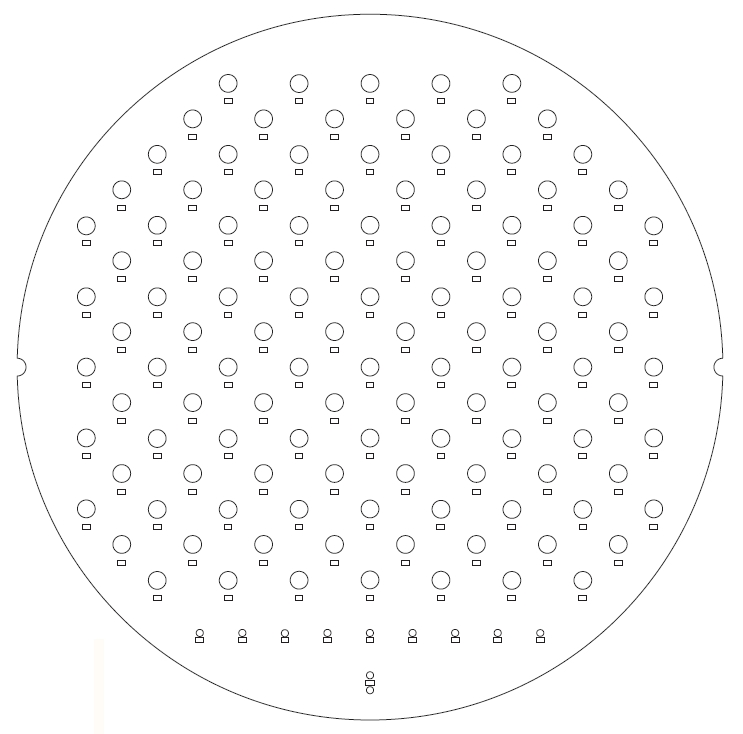
\includegraphics[width=0.8\textwidth]{./dados/figuras/tampo}
    \fonte{MITSUKO, 2016}
    \label{fig:tampo}
\end{figure}

A arquiteta também especifica que o funcionamento da mesa deve ser orientado a eventos, provenientes das seções Controle e Matriz (\autoref{fig:mesa-sup}):

\begin{itemize}[noitemsep]
    \item A mesa sai do modo ocioso ao manter-se a mão sobre a bolinha \emph{Power} por mais de 1s: acende-se o seletor de cores e a mesa passa a interpretar os demais comandos;
    \item Escolhe-se uma cor ao manter-se a mão sobre uma determinada bolinha do seletor de cores por mais de 1s;
    \item Ao passar a mão sobre uma determinada bolinha da seção Matriz, a mesma deve responder com a última cor escolhida;
    \item Uma bolinha da seção Matriz pode ser apagada se a ``cor'' escolhida tiver sido a da bolinha \emph{Power};
    \item Ao manter-se a mão por mais de 3s sobre a bolinha \emph{Power}, todas as bolinhas da seção Matriz devem ser apagadas; e
    \item Ao manter-se a mão por mais de 5s sobre a bolinha \emph{Power}, a mesa entra em modo ocioso: as bolinhas do seletor de cores são apagadas e a mesa passa a ignorar os comandos sobre a Matriz.
\end{itemize}

A partir da especificação acerca do funcionamento, notam-se alguns desafios do ponto de vista do eletrônico/lógico, tais como:

\begin{itemize}
    \item A disposição dos objetos e o tamanho da mesa;
    \item A capacidade de comandar individualmente 129 \emph{LEDs} coloridos (\emph{RGB}), ou seja $129 \times 3 = 387$ canais de cor;
    \item A capacidade de interpretar os níveis lógicos dos 128 sensores;
    \item A capacidade de responder, simultaneamente, aos comandos temporais provenientes de cada sensor.
\end{itemize}

A seleção dos componentes e das ferramentas foi baseada na especificação e nos desafios acima citados, e será discutida a seguir nas demais seções deste capítulo.

\section{SENSOR}
\label{sec:sensor}

A função do sensor é identificar a posição de um objeto, no caso, a mão do espectador, sobre o tampo acrílico, e para manter-se centrado nos objetivos do projeto arquitetônico, a definição do tipo de sensor foi baseada em dois pontos essenciais:

\begin{enumerate}[label=\Roman*.]
    \item O elemento principal do projeto é a luz que flui da bolinha de \emph{ping-pong};
    \item A exposição pode ser levada a diversos lugares e ser instalada nos mais variados ambientes, como museus, escolas, saguões e etc.
\end{enumerate}

A questão (I) implica que o sensor não deve irradiar ondas eletromagnéticas dentro do espectro visível, que vai de $400nm$ a $700nm$ \cite{fundafisica}. Já a questão (II) implica que a instalação será submetida a locais com diferentes graus de iluminação, portanto os sensores devem ser imunes à variação luminosa do ambiente.

Assim sendo, optou-se pelo sensor óptico reflexivo \emph{TCRT5000L}, apresentado na \autoref{fig:sensor}, cujas características relevantes para o projeto são apresentadas na \autoref{tab:sensor}.

\begin{figure}[H]
    \centering
    \caption{Sensor TCRT5000}
    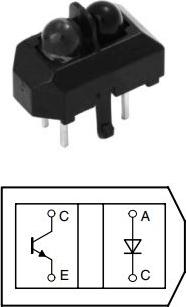
\includegraphics[width=0.24\textwidth]{./dados/figuras/sensor}
    \fonte{\citeonline{datasheet-sensor}}
    \label{fig:sensor}
\end{figure}

\begin{table}[H]
    \centering
    \caption[Principais características do sensor]{Principais características do sensor.
    \label{tab:sensor}}
    \begin{tabular}{|l|l|l|l|l|l|l|}
        \hline
        \textbf{Parâmetro} & \textbf{Condição} & \textbf{Símb.} & \textbf{Mín.} & \textbf{Típ.} & \textbf{Máx.} & \textbf{Unidade} \\     \hline
        \emph{LED} - Corrente direta &  & $I_{F}$ &  & 60 &  & mA \\ \hline
        \emph{LED} - Queda direta de tensão & $I_{F} = 60mA$ & $V_{F}$ &  & 1,25 & 1,5 & V \\ \hline
        \emph{LED} - Comprimento de onda & $I_{F} = 100mA$ & $\lambda_{P}$ & 940 &  &  & nm \\ \hline
        Sensor - Corrente de coletor & \begin{tabular}[c]{@{}l@{}}$@5V$,\\ $I_{F} = 10mA$,\\ $D=12mm$\end{tabular} & $I_{C}$ & 0,5 & 1 & 2,1 & mA \\ \hline
        \begin{tabular}[c]{@{}l@{}}Sensor - Queda de tensão entre\\ coletor-emissor na saturação\end{tabular} & \begin{tabular}[c]{@{}l@{}}$I_{F} = 10mA$, \\ $I_{C}=0,1mA$,\\ $D=12mm$\end{tabular} & $V_{CE_{sat}}$ &  &  & 0,4 & V \\ \hline
    \end{tabular}
    \fonte{\citeonline{datasheet-sensor}}
\end{table}


Trata-se de um sensor reflexivo infravermelho ($\lambda_{P}$), ou seja, opera fora do espectro visível, o que contorna a implicação da questão (I) apresentada anteriormente. Além disso, diferentemente de um sensor passivo, por exemplo um LDR, o TCRT5000 opera irradiando luz e, ademais, também contém filtro óptico embutido, absorvendo somente comprimentos de onda próximas a ($\lambda_{P}$). Essa duas características contornam a implicação da questão (II).

A saída transistorizada permite que o sensor seja interpretado de forma lógica. Sua aplicação (\autoref{fig:sensoraplicacao}) vai desde sensoriamento de \emph{encoders} e posições de ``fim de curso'' até detecção de papéis, cartões, fitas e etc. Foi escolhida a variante ``L'' (\emph{TCRT5000\textbf{L}}) por ser a versão com terminais estendidos.

\begin{figure}[H]
    \centering
    \caption{Aplicação do sensor TCRT5000}
    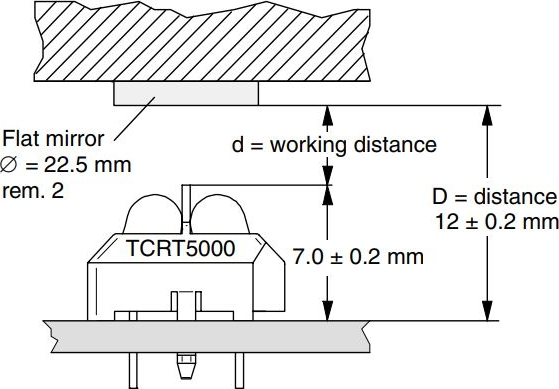
\includegraphics[width=0.5\textwidth]{./dados/figuras/sensor-op}
    \fonte{\citeonline{datasheet-sensor}}
    \label{fig:sensoraplicacao}
\end{figure}

\section{REGISTRADORES DE DESLOCAMENTO}
\label{sec:registradores}

A necessidade de interpretar individualmente os 128 sensores implica na mesma quantidade de entradas do circuito de processamento. Então, optou-se por lidar com entradas virtuais, através de um barramento serial, por meio de registradores de deslocamento. Dessa forma, com poucas GPIOs, o microcontrolador pode interpretar os níveis lógicos de todos os sensores conectados ao barramento.

Devido sua grande difusão no mercado, o registrador de deslocamento escolhido foi o 74HC165. A \autoref{fig:shift-register} apresenta o diagrama funcional do circuito integrado.

\begin{figure}[H]
    \centering
    \caption{Diagrama funcional do 74HC165}
    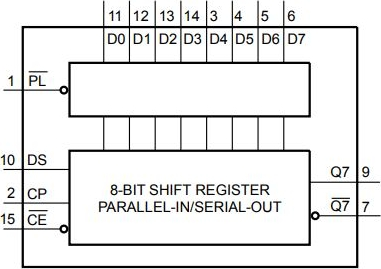
\includegraphics[width=0.5\textwidth]{./dados/figuras/shift-register}
    \fonte{\citeonline{datasheet-shift-register}}
    \label{fig:shift-register}
\end{figure}

Trata-se de um registrador de deslocamento com 8 entradas em paralelo ($D_{N}$) e saídas complementares ($Q_{7}$ e $\overline{Q_{7}}$) em serial. Basicamente, seu funcionamento (\autoref{fig:shift-temporal}) constitui-se na captura instantânea do nível lógico de suas entradas (borda de descida da Entrada Assíncrona de Carga Paralela, $\overline{P_{L}}$) e na transmissão desses valores através de deslocamento ordenado ($D_{7} \rightarrow D_{0}$) na saída serial ($Q_{7}$), nos eventos de borda de subida na entrada de \emph{clock} ($C_{P}$).

\begin{figure}[!htb]
    \centering
    \caption{Diagrama temporal do 74HC165}
    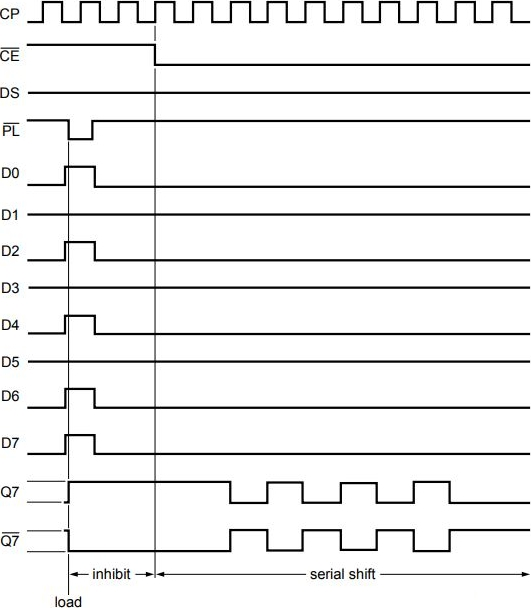
\includegraphics[width=0.6\textwidth]{./dados/figuras/shift-temporal}
    \fonte{\citeonline{datasheet-shift-register}}
    \label{fig:shift-temporal}
\end{figure}

\section{LED}
\label{sec:led}

\textcolor{red}{Protocolo NRZ}

\section{MICROCONTROLADOR}
\label{sec:microcontrolador}

O ESP8266 é o microcontrolador de entrada para a família de 32 bits da fabricante chinesa Espressif Systems. Produzido em escala a partir de 2014, essa família ganhou espaço na área de Internet das Coisas por ser um microcontrolador de baixo custo, de baixo consumo e com suporte à rede 802.11 (\emph{Wi-Fi}). A \autoref{tab:espec-microcontrolador} apresenta as principais especificações do microcontrolador e a \autoref{fig:esp-funcional} apresenta seu diagrama funcional. Cabe aqui ressaltar que toda a parte de radio-frequência é implementada por \emph{hardware}, simplificando o desenvolvimento de aplicações com comunicação sem fio.

\begin{table}[H]
    \centering
    \caption[Especificação do ESP8266]{Especificação do ESP8266.
    \label{tab:espec-microcontrolador}}
    \begin{tabular}{|l|l|}
    \hline
    Alimentação & 3,3\ V \\ \hline
    Consumo & $10\ \mu A - 170\ mA$ \\ \hline
    Memória Flash (externa) & 16\ MB máx. (512\ kB normal) \\ \hline
    CPU & Tensilica L106 32 bits \\ \hline
    \emph{Clock} & $80 - 160\ MHz$ \\ \hline
    RAM & $32\ kB - 80\ kB$ \\ \hline
    GPIOs & 17 (compartilhadas com outras funções) \\ \hline
    ADC & 1 canal (10 \emph{bits} de resolução) \\ \hline
    \emph{Wireless} & Estação, ponto de acesso ou ambos \\ \hline
    \end{tabular}
    \fonte{\cite{book-esp}}
\end{table}


\begin{figure}[!htb]
    \centering
    \caption{Diagrama funcional do ESP8266}
    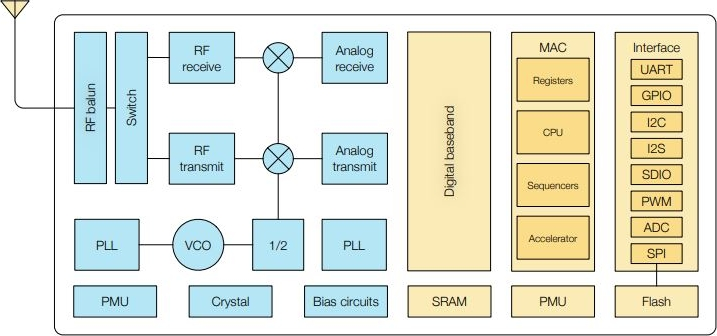
\includegraphics[width=0.9\textwidth]{./dados/figuras/esp-funcional}
    \fonte{\citeonline{datasheet-esp}}
    \label{fig:esp-funcional}
\end{figure}

Embora a comunicação sem fio não fizesse parte das especificações do projeto arquitetônico original, a equipe concordou com a possibilidade de implementá-la em uma aplicação futura. Esse foi o ponto decisivo para a escolha do ESP8266. Assim, a Mesa de Bolinhas poderá ganhar novas funcionalidades sem haver a necessidade de alteração no \emph{hardware}. Isso será discutido na \autoref{sec:trabalhosFuturos}.

Entre os diversos módulos que incluem o ESP8266, optou-se pelo ESP-12, por ser o que dispõe a maior quantidade de \emph{GPIOs} (9 ao todo). A \autoref{fig:esp-12} apresenta sua placa. Convém salientar que este módulo já conta com memória \emph{Flash} (4MB) e antena \emph{microstrip}.

\begin{figure}[H]
    \centering
    \caption{Módulo ESP-12}
    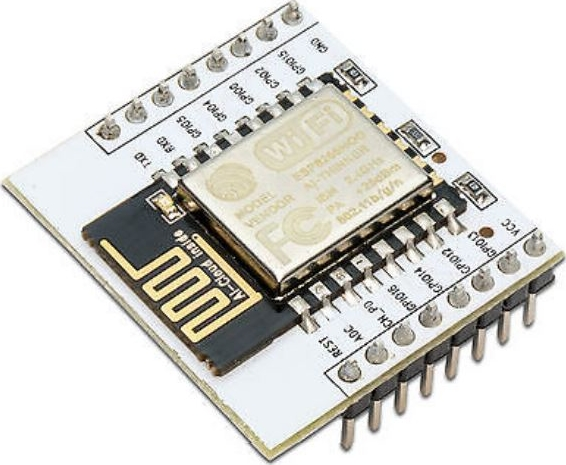
\includegraphics[width=0.4\textwidth]{./dados/figuras/esp-12}
    \fonte{\cite{book-esp}}
    \label{fig:esp-12}
\end{figure}

\section{\emph{FRAMEWORK}}
\label{sec:framework}

Sming é um \emph{framework} de código aberto, nativo para a família de microcontroladores ESP8266, desenvolvido na linguagem {C++} e com foco em alta eficiência em desempenho e em uso de memória.

Diferente de outros \emph{frameworks} baseados em laço-infinito, a estrutura do Sming é baseada em eventos temporais: as tarefas do usuário são escaladas em uma tabela de tempo. Isso o aproxima de uma das funcionalidades de um Sitema Operacional de Tempo Real, embora não haja, obviamente, um gerenciamento de recursos. Porém, o fato de poder-se escalar as tarefas em uma janela de tempo simplifica a implementação da especificação deste projeto, uma vez que, basicamente, sua funcionalidade também é baseada em eventos temporais, como apresentado no começo do capítulo (\autoref{sec:matrizLed}).

Por tratar-se de uma plataforma de código aberto, este \emph{framework} conta com uma vasta contribuição da comunidade, com uma API de \emph{hardware} robusta e diversas bibliotecas nativas, tais como \emph{bootloader}, sistema de arquivos (SPIFFS), atualização sem fio de \emph{firmware} (OTA) e uma extensa pilha assíncrona de rede (TCP, UDP, \emph{WebSockets} e etc). Esses recursos são úteis para a continuidade do projeto, discutida na \autoref{sec:trabalhosFuturos}.
